\section{Statistical Models for Epidemiological Rates}
\label{theory-rate_model}

The key to connecting the systems dynamics model from
Chapter~\ref{theory-system_dynamics} to the evidence base collected
through systematic review is the \emph{rate model}.  This is a
statistical model, which has its core features defined by its
likelihood function.  By \emph{likelihood function}, I mean a
probability density function that assigns a value for the likelihood
of every possible (rate value, uncertainty)-pair for each setting of
the model parameter.  An examples will make this clearer, so I turn
now to the meta-analysis of population prevalence of schizophrenia in
adult males.  The forest plot in
Figure~\ref{fig:theory-rate_model-schiz_forest} shows the results of
combining $<<len(d['schiz_forest.json|dexy']['r'])>>$ studies using
$7$ different rate models.  As the figure demonstrates, the choice of
rate model can have a huge effect on the estimated uncertainty, and
can have a noticable effect on the estimated median as well. The
models I displayed produce point estimates ranging from
$<<d['schiz_forest.json|dexy']['min_est']>>$ to
$<<d['schiz_forest.json|dexy']['max_est']>>$, and uncertainty
intervals with widths ranging from
$<<d['schiz_forest.json|dexy']['min_spread']>>$ to
$<<d['schiz_forest.json|dexy']['max_spread']>>$.

In what follows, I will develop a collection of rate models, starting
with the simplest and then increasing complexity, while identifying
the benefits and drawbacks of each.  The models to come, in order, are
the binomial model, the beta-binomial model, the poisson model, the
negative binomial model, and three variants of the normal
model.

\begin{figure}
\begin{center}
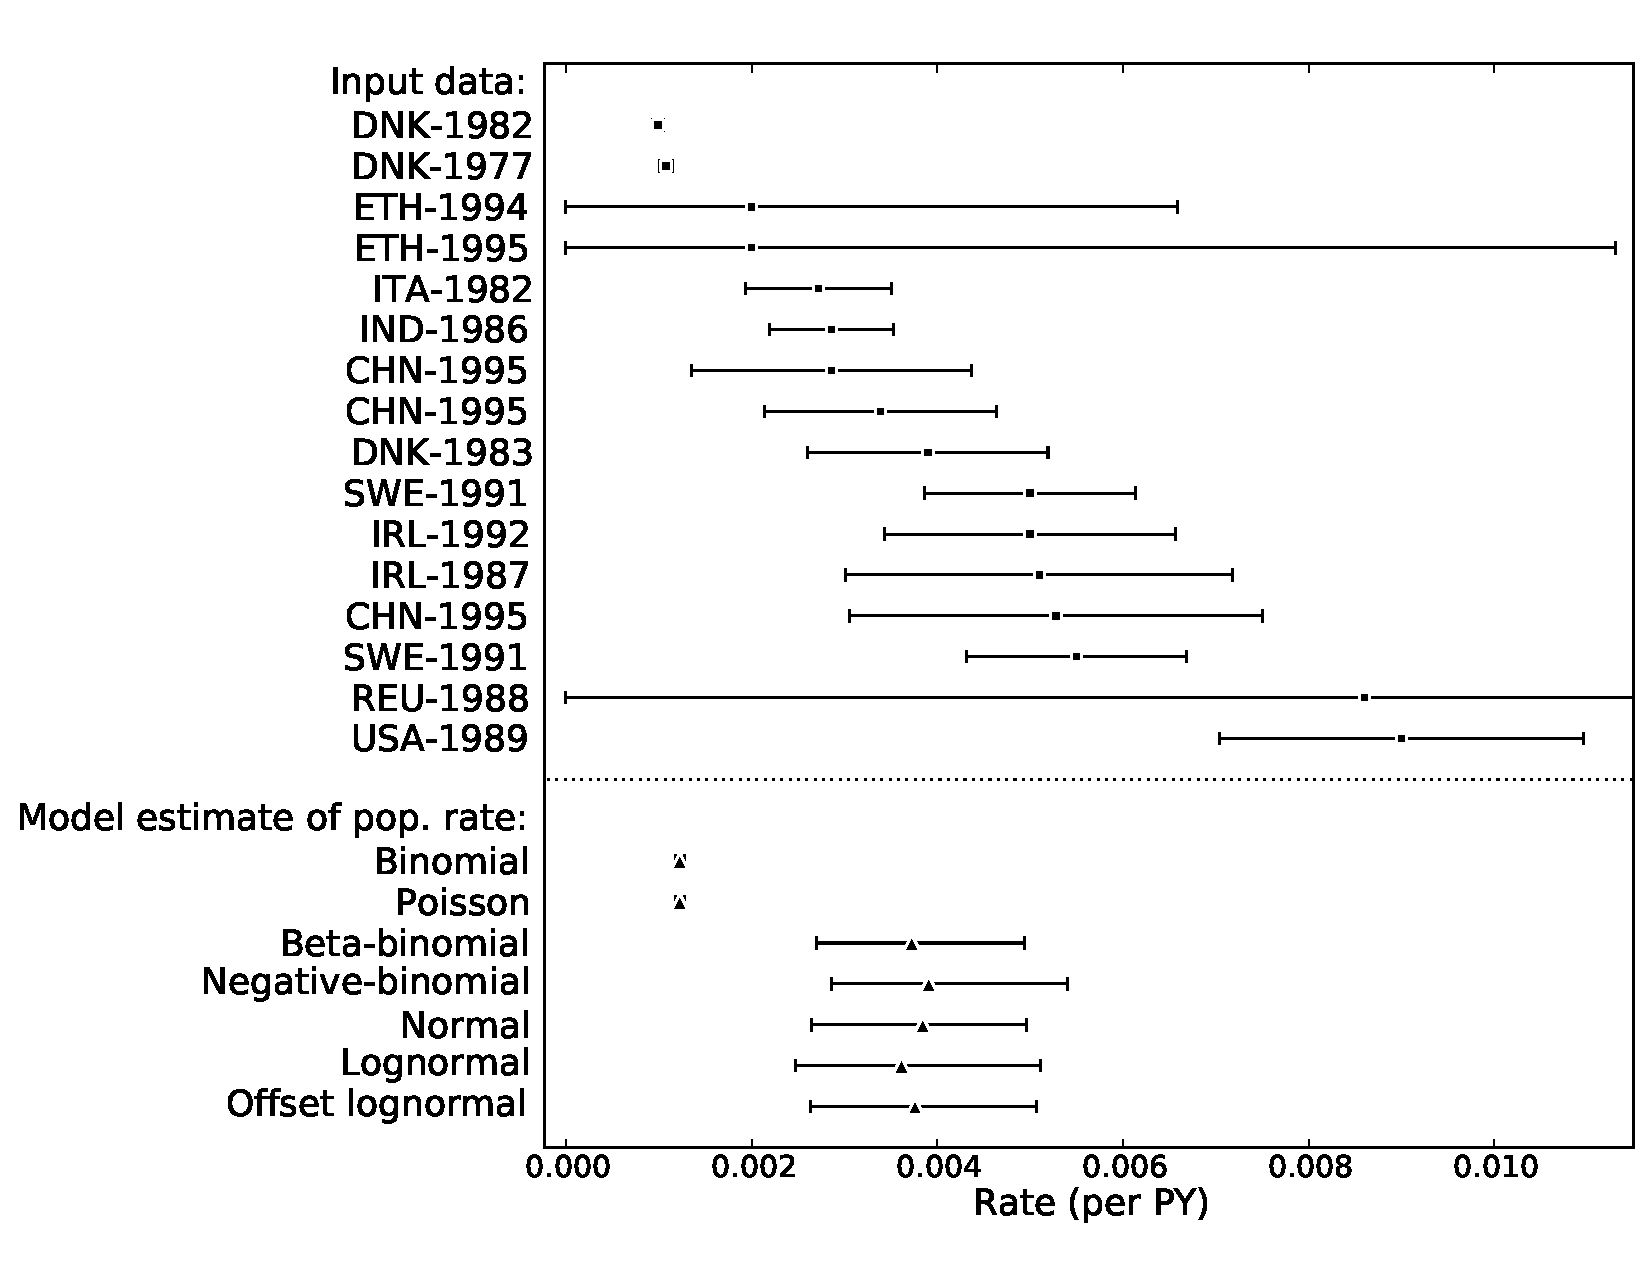
\includegraphics[width=\textwidth]{schiz_forest.pdf}
\end{center}
\caption{Forest plot summarizing $7$ alternative models for
  meta-analysis of adult male schizophrenia prevalence at
  population-level.  The median estimates range from
  $<<d['schiz_forest.json|dexy']['min_est']>>$ to
  $<<d['schiz_forest.json|dexy']['max_est']>>$, and the width of the
  $95\%$ HPD interval ranges from
  $<<d['schiz_forest.json|dexy']['min_spread']>>$ to
  $<<d['schiz_forest.json|dexy']['max_spread']>>$.}
\label{fig:theory-rate_model-schiz_forest}
\end{figure}

\subsection{Binomial Model}
My conceptually simplest model for rate data was built from the
binomial random variable, which follows the probability distribution
\[
\Pr[X=k\given n,\pi] = \binom{n}{k}\pi^n(1-\pi)^{n-k}
\]
I've used greek to emphasize that $\pi$ is the parameter, while $n$
and $k$ are data.

Although this equation may appear opaque, the intuition behind it is
simple: $n$ individuals were tested for a disease, and $k$ tested
positive. The formula then follows from the assumption that each
individual tested positive with probability $\pi$, and that 
knowing about the test results of any subset of individuals gives me
no information about what the test results the others were
(these events are ``independent'').

This distribution inspires a computationally tractable and
theoretically appealing rate model for a observed population rate of
$r$ from a population of size $n$:
\[
\dens(p,n\given \pi) \propto \pi^{\lfloor rn \rfloor}(1-\pi)^{\lceil (1-r)n \rceil}.
\]
Note that it is not necessary to include the term $\binom{n}{nr}$,
because this does not depend on the model parameter $\pi$. There is a
constant of proportionality, which is necessary to make this rate
model truely a probability density function for any $\pi$, but happily
I will never need to know this constant, and I have use the ``proportional to''
symbol $\propto$ instead of equality to emphsize this fact.

The funnel plot in Figure~\ref{fig:theory-rate_model-binom_funnel}
shows the predictive distribution of this rate model for $\pi=<<
d['binomial_model.json|dexy']['pi_binomial_funnel'] >>$.  It also shows
the potential problem with this approach: the data gathered by
systematic review are often much more dispersed than this
distribution predicts.

\begin{figure}[ht]
\begin{center}
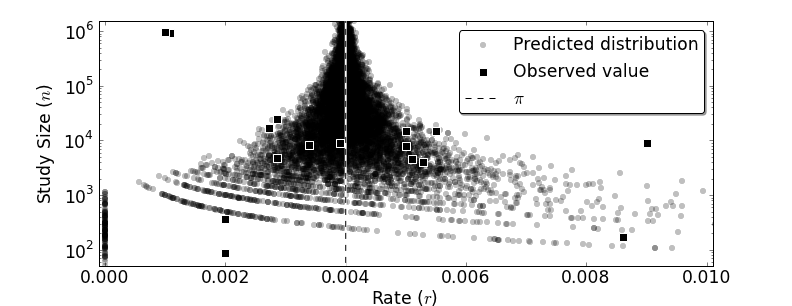
\includegraphics[width=\textwidth]{binomial-model-funnel.png}
\end{center}
\caption{Funnel plot showing predictive distribution for the binomial
  rate model with
  $\pi=<<d['binomial_model.json|dexy']['pi_binomial_funnel']>>$ (shown in
  blue), with data from systematic review for adult male schizophrenia
  prelvanece overlaid for comparison (shown in green).}
\label{fig:theory-rate_model-binom_funnel}
\end{figure}

All models are wrong, of course, so why does this model require
refinement? The answer is that is leads to unreasonably high
confidence when modeling noisy data.  If a study of
$<<d['binomial_model.json|dexy']['pop_A_N']>>$ people from in
subpopulation A finds prevalence of
$<<d['binomial_model.json|dexy']['pop_A_prev']*1000>>$ per thousand and
a study of $<<d['binomial_model.json|dexy']['pop_B_N']>>$ people in
subpopulation B finds $<<
d['binomial_model.json|dexy']['pop_B_prev']*1000 >>$, then the
binomial model predicts that a study of
$<<d['binomial_model.json|dexy']['pop_C_N']>>$ people in subpopulation
C will have prevalence of
$<<d['binomial_model.json|dexy']['pop_C_prev_per_1000']>>$, with
$95\%$ HPD interval
$<<d['binomial_model.json|dexy']['pop_C_ui_per_1000']>>$.  I have
no problem with the point estimate.  Picking the mean of the two
populations seems just right.  But the uncertainty interval lacks face
validity.  It would be much more reasonable to have an uncertainty
interval as large as $[1,7]$, instead of one as small as this.

One way to formalize this objection is through the posterior
predictive check, an in-sample goodness-of-fit test that can be done
graphically.  Figure~\ref{fig:theory-rate_model-binom_ppc} shows the
posterior predictions of the binomial model when it is fit to the
adult male schizophrenia dataset, together with the data itself.  The
model predictions are clearly compressed, and trusting the results of
such a model will lead to inappropriate certainty in the face of noisy
data.

\begin{figure}[ht]
\begin{center}
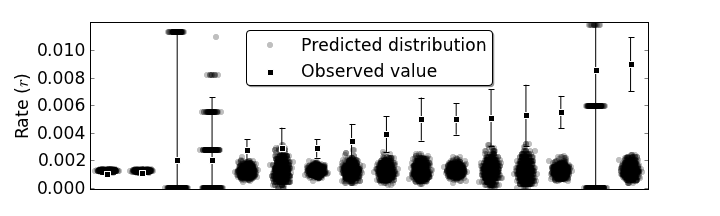
\includegraphics[width=\textwidth]{binomial-model-ppc.png}
\end{center}
\caption{Posterior predictive check for binomial model fit to adult
  male schizophrenia data.  Blue shows 1000 draws from the posterior
  distribution of the binomial model, and green shows the input data.}
\label{fig:theory-rate_model-binom_ppc}
\end{figure}




\subsection{Beta-binomial model}
\label{beta-binomial-model}
A theoretically appealing extension to the binomial model (which also
does not work for my purposes) is the beta-binomial model.  I will
develop it in this section, to motivate the following sections.

Formally, the beta binomial random variable is given by the following
probability distribution
\begin{align*}
\Pr[X = k\given n, \alpha, \beta] 
  &= \int_{\pi}\dens(\pi\given \alpha, \beta) \binom{n}{k}\pi^k(1-\pi)^{n-k}
d\pi\\
\dens(\pi\given \alpha, \beta) &\propto \pi^{\alpha-1}(1-\pi)^{\beta-1}
\end{align*}

The intuition behind this model is simpler than the equation, however.
As in the binomial model, each individual tests positive for the condition independently
with a probability $\pi$, but now $\pi$ itself is a random variable,
distributed according to a beta distribution with parameters $\alpha$
and $\beta$. The beta distribution is given by 
\[
\dens(\pi\given \alpha, \beta) =
\frac{\Gamma(\alpha+\beta)}{\Gamma(\alpha)\Gamma(\beta)}\pi^{\alpha-1}(1-\pi)^{\beta-1}
\]
and has a high degree of flexibility.  It also always takes values
between zero and one, making it an appropriate distribution for a
probability.  Figure~\ref{fig:theory-rate_model-beta} shows the
probability density of the beta distribution for several combinations
of $\alpha$ and $\beta$.
\begin{figure}[ht]
\begin{center}
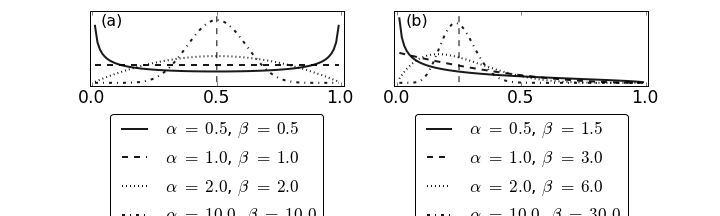
\includegraphics[width=\textwidth]{beta-distribution.png}
\end{center}
\caption{Probability density for the beta distribution for a range of
  $\alpha$ and $\beta$ values. Dashed black line shows expected value,
which is $.5$ for all distribution in a) and $.25$ for all in b).}
\label{fig:theory-rate_model-beta}
\end{figure}

The beta binomial distribution inspired the following rate model for
an observed population rate of $r$ from a population of size $n$:
\[
\dens(r,n\given \alpha, \beta) \propto \int_{\pi}
\pi^{\alpha-1}(1-\pi)^{\beta-1} \pi^{\lfloor rn\rfloor} (1-\pi)^{\lceil (1-r)n\rceil}
d\pi.
\]

This model extends the binomial model in a way analogous to how a
random effects model in linear regression.  By introducing an
additional dimension in to the parameter space, it is able to capture
the dispersion beyond the binomial model that I have observed
empirically in funnel plots of real data
(Figure~\ref{fig:theory-rate_beta-binomial-funnel} shows the beta
binomial funnel plot, as well as the posterior predictive check for
this model on the same data as used in
Figure~\ref{fig:theory-rate_model-binom_ppc}.

\begin{figure}[ht]
\begin{center}
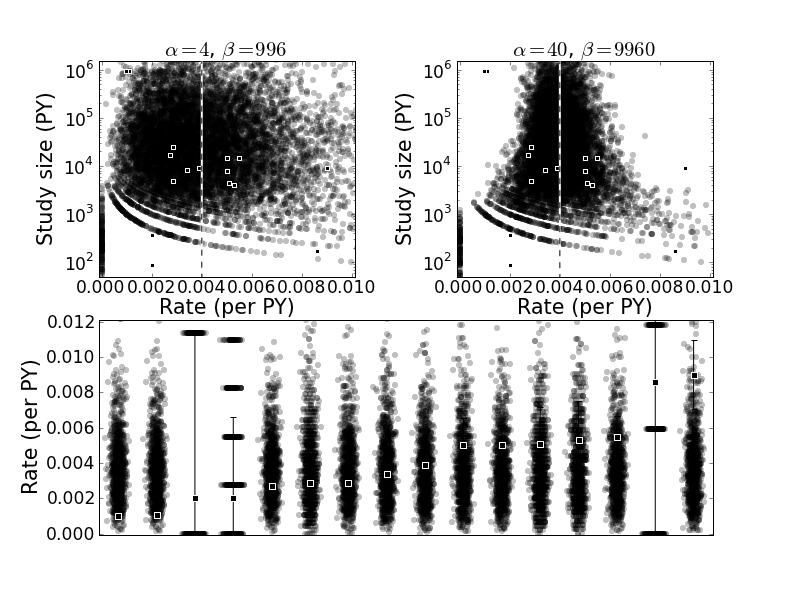
\includegraphics[width=\textwidth]{beta-binomial-funnel.png}
\end{center}
\caption{Funnel plot and posterior predictive check for beta binomial model.}
\label{fig:theory-rate_beta-binomial-funnel}
\end{figure}

This model addresses the theoretical shortcoming raised in the
previous section: if studies of
$<<d['beta_binomial_model.json|dexy']['pop_A_N']>>$ people show prevalences
of $<<d['beta_binomial_model.json|dexy']['pop_A_prev']*1000>>$ and
$<<d['beta_binomial_model.json|dexy']['pop_B_prev']*1000>>$ per thousand,
then the posterior distribution of the beta binomial model has mean
$<<d['beta_binomial_model.json|dexy']['pop_C_prev_per_1000']>>$ with 95\%
HPD interval $<<d['beta_binomial_model.json|dexy']['pop_C_ui_per_1000']>>$,
which seems quite reasonable.

The great shortcoming of the beta binomial model is computational.  As
will be elaborated in Chapter~\ref{theory-numerical_algorithms}, there
is no closed-form solution to the integral in the probability density
for the beta binomial model.  Evaluating it requires introducing a
latent variable for each of the data points in the likelihood.  This
simply had too much cost for the numerical algorithms and
computational infrastructure available.  So my search
continued.

\subsection{Other count models}
There are two traditional approximations to the binomial distribution,
depending on how large $k$ is in relation to $n$.  When $k/n$ is
large, the normal distribution is used, and when $k/n$ is small, the
binomial is similar to the Poisson distribution.

Since I expect to usually be in a ``small $k/n$'' setting, I will not
develop the normal model in detail now, although in the next section I
will develop to model based on monotonic transformations of the normal
distribution which include a normal model as a special case.

The Poisson distribution is given by the the equation
\[
\Pr[X=k] = \frac{\lambda^k e^{-\lambda}}{k!},
\]
and it can be understood intuitively as the number of times a
``memoryless'' event occurs in a unit time period.  Setting $\lambda =
\pi n$ produces an approximation to the binomial distribution, which
is quite accurate for large $n$ and small $k$.
Figure~\ref{fig:theory-rate_model-poisson_approx_to_binom}
demonstrates how precise this approximation can be when approximating
a binomial distribution with
$n=<<d['poisson_model.json|dexy']['n_small']>>$ and
$\pi=<<d['poisson_model.json|dexy']['pi_true']>>$.

\begin{figure}
\begin{center}
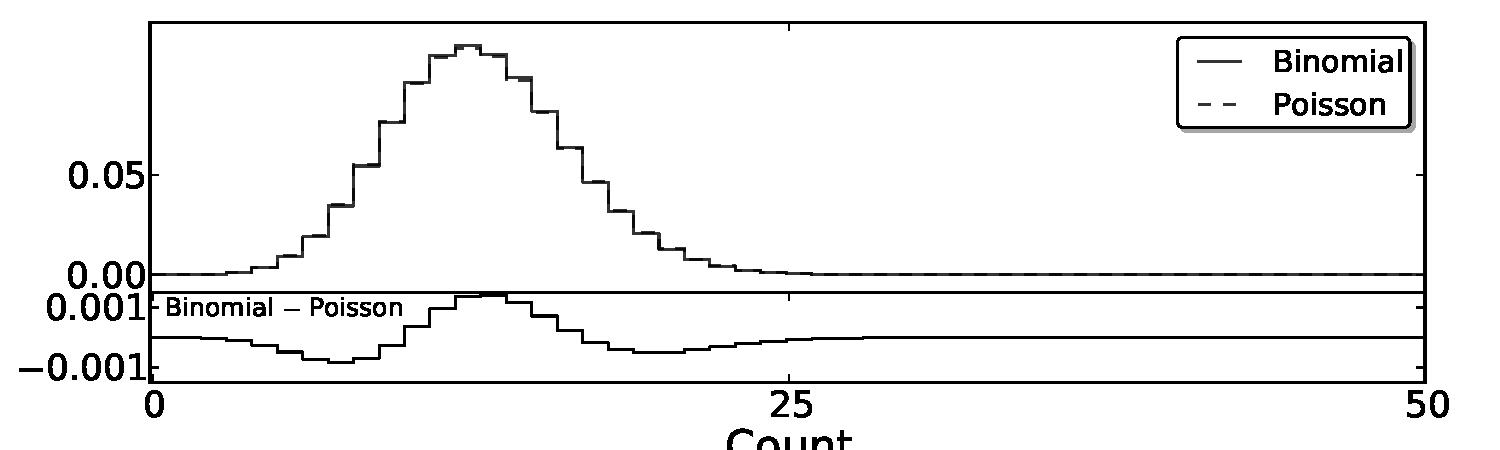
\includegraphics[width=\textwidth]{poisson_approx_to_binom.png}
\end{center}
\caption{The Poisson distribution approximates the binomial
  distribution very closely. Here a binomial distribution with
  $n=<<d['poisson_model.json|dexy']['n_small']>>$ and
  $\pi=<<d['poisson_model.json|dexy']['pi_true']>>$ is approximated by
  a Poisson distribution with parameter
  $\lambda=<<d['poisson_model.json|dexy']['n_small'] *
  d['poisson_model.json|dexy']['pi_true']>>$.  The difference between
  the distributions is shown in the lower panel, since the curves in
  the upper panel are almost indistinguishable by eye.}
\label{fig:theory-rate_model-poisson_approx_to_binom}
\end{figure}

Because of the similarity of these distributions, my Poisson model,
which defined as
\[
\dens(r,n\given \pi) \propto (\pi n)^{\lfloor rn\rfloor} e^{-\pi n},
\]
is quite similar to the binomial model defined above.  It is also subject to all of the concerns raised about the
binomial model regarding inappropriately low levels of uncertainty
when modeling rates with non-sampling variation at the level typically
gathered in systematic review.

There is one key benefit to this model, compared to the binomial and
beta-binomial models, however.  The Poisson model assigns a
theoretically justified and non-zero likelihood to rates of more than
one.  Although prevalence is always less than one, it is theoretically
possible to have incidence rates more than one, and remission rates
are often more than one (per person-year).

Another benefit from this approach is to be found in its
over-dispersed variant.  This distribution
is called the negative binomial distribution (named after the formula
that the proves it does indeed sum to one).  Unlike the beta-binomial
distribution, it \emph{does} have a closed form (if you consider the gamma function ``closed''):
\[
\Pr[X = k\given \pi, \delta] = \frac{\Gamma(k+\delta)}{\Gamma(\delta)k!}
\left(\frac{\delta}{\pi+\delta}\right)^\delta \left(\frac{\pi}{\pi+\delta}\right)^k
\]

However, this closed form obscures the intuition behind the negative
binomial distribution, which is quite similar to the intuition behind
the beta-binomial distribution (but less clear from its
name). Through a bit of algebra, the negative binomial distribution can
be represented as a hierarchical model, where the observed data comes
from a Poisson distribution, and the parameter of the Poisson
distribution is itself a random variable that comes from a gamma
distribution:
\begin{align*}
X\given \pi &\sim \Poisson(\pi)\\
\pi &\sim \GammaDist(\mu, \delta)
\end{align*}
Here the Gamma distribution is defined by (TK reparameterize to match above)
\[
\dens(x; k,\theta) =
x^{k-1} \frac{e^{-x/\theta}}{\theta^k \, \Gamma(k)}.
\]
Through this lens, the negative binomial model can be interpreted as a
nature adaptation of the traditional random effects model in linear
regression to the Poisson case, where each observation comes from a
different Poisson model and the Poisson parameter of these models are
all drawn from a common Gamma distribution.

Thus a rate model based on it provides benefits in handling
non-sampling variation similar to those demonstrated for the beta
binomial distribution above, but in a formulation that is much less
demanding computationally.  The negative-binomial rate model for
observing a rate of $r$ in a population of size $n$ is:
\[
\dens(r,n\given \pi, \rho) \propto \frac{\Gamma(\lfloor rn\rfloor+\rho)}{\Gamma(\rho)} (1-\pi)^\rho \pi^{rn}.
\]

A difficultly I have observed in practice with the negative binomial
model is in the realm of numerical algorithms.  My experience has been that these
likelihoods lead to models that are simply harder to fit than
traditional normal models.  Nonetheless, the negative binomial model
has been the primary tool in the likelihod modeling for the
applications to be presented in Chapters~\ref{practice-all-examples}.

Chapter~\ref{TK} will examine the properties of numerical algorithms
for fitting the negative binomial model in more detail, but one
approach which has helped substantially is imposing an informative
prior on the over-dispersion parameter of the negative binomial
distribution.  Because it seems unreasonable to impose a very
informative prior on the over-dispersion parameter, I have limited the
possibilities to augmenting the hierarchical formulation of the
negative binomial model above with the following:
\[
\log_{10} (\delta-.5) \sim \Normal\left(\mu_{\log\delta}, .25^2\right),
\]
with $\mu_{\log\delta} = 1, 2, 3$.  The results of adding this
prior are contrasted with the results vanilla negative binomial model
(with an uninformative prior on $\delta$) in
Figure~\ref{fig:theory-rate_model-neg_binom_priors}, which shows that
a belief a priori that the observations is more over-dispersed leads
to a posterior estimate where the predicted rate have more
uncertainty, as expected.

\begin{figure}
\begin{center}
\includegraphics[width=\textwidth]{neg_binom_priors.pdf}
\end{center}
\caption{Forest plot of a simulation experiment demonstrating the
  effect of a weakly informative prior on the negative binomial model
  posterior.  Sixteen data points simulated from a negative binomial
  distribution are fit with negative binomial models, with $5$
  different priors on the dispersion term $\delta$.  The informative
  prior of $\delta = \infty$ reduces the negative binomial model to
  the poisson model, and for this case the uncertainty interval does
  not contain the truth.  All of the weakly informative priors do
  contain the truth, however.  Replicating this simulation
  $<<d['neg_binom_sim.json|dexy']['replicates']>>$ times yielded mean
  bias of
  $\E[\pi_{\true}-\pi_{\median}]=<<d['neg_binom_sim.json|dexy']['bias']['pi']>>$
  and root mean squared error of
  $\RMSE[\pi_{\true}-\pi_{\median}]=<<d['neg_binom_sim.json|dexy']['rmse']['pi']>>$;
  the uncertainty interval contained the $\pi_{\true}$ value with probability
  $<<d['neg_binom_sim.json|dexy']['percent_coverage']['pi']>>$.}
\label{fig:theory-rate_model-neg_binom_priors}
\end{figure}

\subsection{Transformed normal models}
\label{transformed-normal-models}
Some epidemiological data is not count data at all.  Duration studies
and studies measuring the relative risk of mortality are two that come
up frequently in systematic review.  For duation data, a normal model
has been quite sufficient, and a log-normal model has proven
appropriate for modeling relative risk data, which can be thought of
as a ratio of count variables.

Transformed normal models have also been used for mortality rates in
the past [ref including GK TK], and are worthy of continued consideration for
modeling the incidence, prevalence, remission, and mortality as an
alternative to the negative binomial.

In this section, I will develop a general transformed normal model,
and compare it to the negative binomial model.  The adjective
``transformed'' refers to a function which I will keep quite general
for now, requiring it only to be increasing and differentiable,
i.e. for any $x > y$ the transformation $f$ must have $f(x) > f(y)$
and $f'(x)$ must be defined.  Then transformed normal model will be
derived from the normal distribution, defined by the probability
density
\[
\dens(x\given \pi, \sigma) \propto \frac{1}{\sigma} \exp\left\{ -\frac{(x-\pi)^2}{2\sigma^2} \right\}.
\]

For any increasing, differentiable function $f$, this distribution can be converted to
an $f$-transformed normal model with probability density
\[
\dens(r,s\given \pi, \sigma, f) \propto \exp\left\{-\frac{\left(f(r)-f(\pi)\right)^2}{2\left((sf'(r))^2+\sigma^2\right)}\right\},
\]
where $s$ is the standard error of the rate $r$, which is more
convenient that the effective sample size $n$ in this case. The
denominator of the exponent deserves some additional discussion.  For
the identity function $f(x) = x$, the derivative $f'(x) = 1$, and the
denominator simplifies to $2(s^2 + \sigma^2)$, a familiar ``inverse
variance'' weighting where $\sigma$ is a random effect to account for
over-dispersion.  When $f$ is a more complicated function, the term
$sf'(r)$ approximates the standard error of the transformed value
$f(r)$.  Although more sophisticated approximations are possible,
experience dictates that the non-sampling variation (parameterized by
$\sigma$) is always larger than the chance variation, so a simple
approximation of the chance variation is sufficient.

Some common transformations $f$ used in related work yield the
lognormal model ($f(x) = \log x$) the logit model ($f(x) = \logit x$)
and the probit model ($f(x) = \probit x$).  All of these approaches
have a significant drawback, however.  The transform is not defined
for $x=0$, so these models cannot use data showing rates of zero.
There are two common methods to fix this, dropping all zeros, and
adding a small offset.  Dropping measurements of zero is clearly
problematic, as it leads to systematic bias in the data that remains
and produces estimates larger than they should be.  This is especially
true for high quality studies which focus on the age pattern of a
disease, where it is quite reasonable for some age groups to have zero
cases observed.  The effect of dropping zeros is to overestimate the
rates in these age groups.

Adding a small amount, such as $0.5$ is an alternative solution, and
indeed, this is the approach taken for cause-specific mortality estimation
in GK [ref TK].  The selection of the offset can appear ad hoc,
however.

Within the framework of the transformed normal model, there is
room to put the solution on firm theoretical foundations.  For
example, by taking $f_\zeta(x) = \log(x + \zeta)$, I obtained the
``offset log transformed model'', which does allow rates of zero,
simply by taking a positive value for $\zeta$.  This model will not be
used extensively in the example application to come later in this
book, but it seems like a promising approach.  It is particularly
appealing in the way it decomposes the non-sampling variation into an
additive error $\zeta$ and a multiplicative error $\sigma$, and I
expect that it will prove useful in the future.  For completeness,
here is the probability density for the offset log transformed model:
\[
\dens(r,s\given \pi, \sigma, \zeta) \propto
\exp\left\{-\frac{\left(\log(r+\zeta)-\log(\pi+\zeta)\right)^2}{2\left(\left(\frac{s}{r+\zeta}\right)^2+\sigma^2\right)}\right\}.
\]

\subsection{Lower-bound data model}
Cause-specific mortality rates are a special case among the
epidemiological rates available for integrative systems modeling of
disease in a population.  These data come from carefully processing of
vital registration system output, from verbal autopsy stdies, and from
some other sources. But unlike incidence, prevalence, and remission
data, there is no rate or ratio in the compartmental model that
corresponds directly to this quanbtity.  This is because of the ``one
death has one cause'' mantra of biomedical theory.  The excess
mortality rate in the system dynamics model from Chapter TK is not
entirely compatible with this idea.

Cause-specific mortality data nonetheless provides \emph{some}
information, and should be used in an integative model if it is
available, especially if other sources are sparse and noisy (they
always are, in my experience).  By decomposing the excess mortality
into part that is ``cause-of-death mortality'' and residual excess
mortality, i.e. $f = f_{cod} + f_{non}$, it follows that $\CSMR =p
\cdot f_{cod} \leq p\cdot f$, so the following lower bound model is
appropriate:
\[
\dens(\CSMR \given \pi,\delta)
=
\begin{cases}
\calD(\CSMR, \pi, \delta), &\qquad\text{if } \pi-\CSMR \geq 0;\\
\calD(\pi, \pi, \delta), &\qquad\text{otherwise.}
\end{cases}
\]

\subsection{Data values of zero}
Rates with measured value of zero can present a particular challenge
for some statistical models, and are worthy of careful investigation.
As discussed in Section~\ref{transformed-normal-models} above, there
are a number of ad hoc approaches that have been developed to allow
data that includes rates of zero to be fit in models that do not allow
zero rates explicitly, such as dropping all of the observations with
value zero, or replacing them by a small, but non-zero value.
However, it is clear that these approaches will introduce bias to the
estimates [refs TK].

TK challenges of coming up with effective sample size for data with
value zero found in systematic review, and some potential approaches
for addressing this, including the failed approach of using the
standard error from the normal approx to the binomial.

Fortunately, all of the count models described above allow data with
zero values to be included without requiring an ad hoc modifications.
Figure~\ref{zero-forest} shows how all of these models perform for a
simulated data set of prevalence data for a rare condition that has
population prevalence of
$<<d['zero_forest.json|dexy']['pi_true']*10000>>$ in $10000$.  Since
the simulated studies of this disease range in sample size from
$n=<<d['zero_forest.json|dexy']['n_min']>>$ to
$n=<<d['zero_forest.json|dexy']['n_max']>>$, it is expected that some
of the smaller studies will find no individuals with the condition.
To make things even harder for the models, I have ``inflated'' the
number of zero studies, by deterministically including $4$ studies
which measured prevalence levels of zero.

A statistical model with appealing theoretical foundations that
explicitly models this ``zero-inflation'' phenomenon is the
zero-inflated beta binomial model, which is even less efficient than
the beta binomial model that was considered in
Section~\ref{beta-binomial-model}.  It augments the beta binomial
model with an additional parameter $\phi$, and uses a mixture
likelihood where each rate has value $0$ with probability $\phi$ and
value given by a beta binomial distribution (which may also have value
$0$) with probability $1-\phi$.  Formally, the zero-inflated beta
binomial distribution is defined by
\[
\dens(r,n\given \alpha, \beta, \phi) \propto \begin{cases}
(1-\phi)\int_{\pi}
\pi^{\alpha-1}(1-\pi)^{\beta-1} \pi^{\lfloor rn\rfloor}
(1-\pi)^{\lceil (1-r)n\rceil}
d\pi, &\quad\text{if } r > 0;
\\
\phi + (1-\phi)\int_{\pi}
\pi^{\alpha-1}(1-\pi)^{\beta-1}
(1-\pi)^{n}
d\pi, &\quad\text{if } r = 0.
\end{cases}
\]

\begin{figure}
\includegraphics[width=\textwidth]{zero_forest.pdf}
\caption{Forest plot comparing models fit to simulated data for a rare
  disease.  The simulation inflated the number of observed zeros to
  challenge the models.}
\label{zero-forest}
\end{figure}




\subsection{Summary and Comparison}
This section has developed $7$ alternative rate models, all with
benefits and drawbacks.  The binomial model is simple and
theoretically appealing, but does not handle non-sampling variation,
producing over-confident estimates in the face of noisy data.  The
beta binomial model deals with over-dispersion through a theoretically
appealing extension to the binomial model, but it is too
computationally demanding to use in my applications.  The poisson
model is a close approximation to the binomial model, and has all of
the drawbacks except it can handle rates greater than 1, which is
important for modeling remission rates.  So it is the negative
binomial model, which extends the poisson model analogously to the way
the beta binomial model extends the binomial model that I have settled
on for most of the applications to follow, using it to model
incidence, prevalence, remission, excess-mortality, and cause-specific
mortality. It is not as ammenable to analysis as I would like however,
and sometimes benefits from weakly informative priors on the
over-dispersion parameter, an undesirable feature that slows down
analysis by requiring sensitivity analysis.  Transformed normal models
are a promising alternative approach, and I have used the normal model
for duration data in some of the following examples, as well as
the lognormal model for standardized mortality rate data and relative
mortality risk data. The offset log transformed model seems
particularly promising as an alternative to the negative binomial
model, and understanding its statistical and computational
characteristics is a promising direction for future research.

TK some sort of comparison: simulation study? posterior predictive
checks? something analogous to SMART counties in small areas
estimation?
